We start off by performing unsupervised learning in the form of clustering analysis on the data. As seen in Figure \ref{fig:dendogram}, we choose to cut at height 13. This leaves us with few clusters in varying in size, which might not be a bad thing, depending on the data. But, we get one very large cluster and few smaller. If we were to have chosen a smaller height, we would have many small clusters, perhapse too many. There is a tradeoff here of having large clusters, that don't really say much about the data, while too small clusters defeats the purpose of clustering (by e.g. having clusters with single data points.)



We don't really get anything exciting with our ratios (neither close to one or zero), not even at height 7, which  probably means that K nearest neighbors will not perform too well and that it in general might be difficult to categorize migrators with a model, since the stars seem to have the same attributes for both migrators and non-migrators.

\begin{figure}[h!]
    \centering
    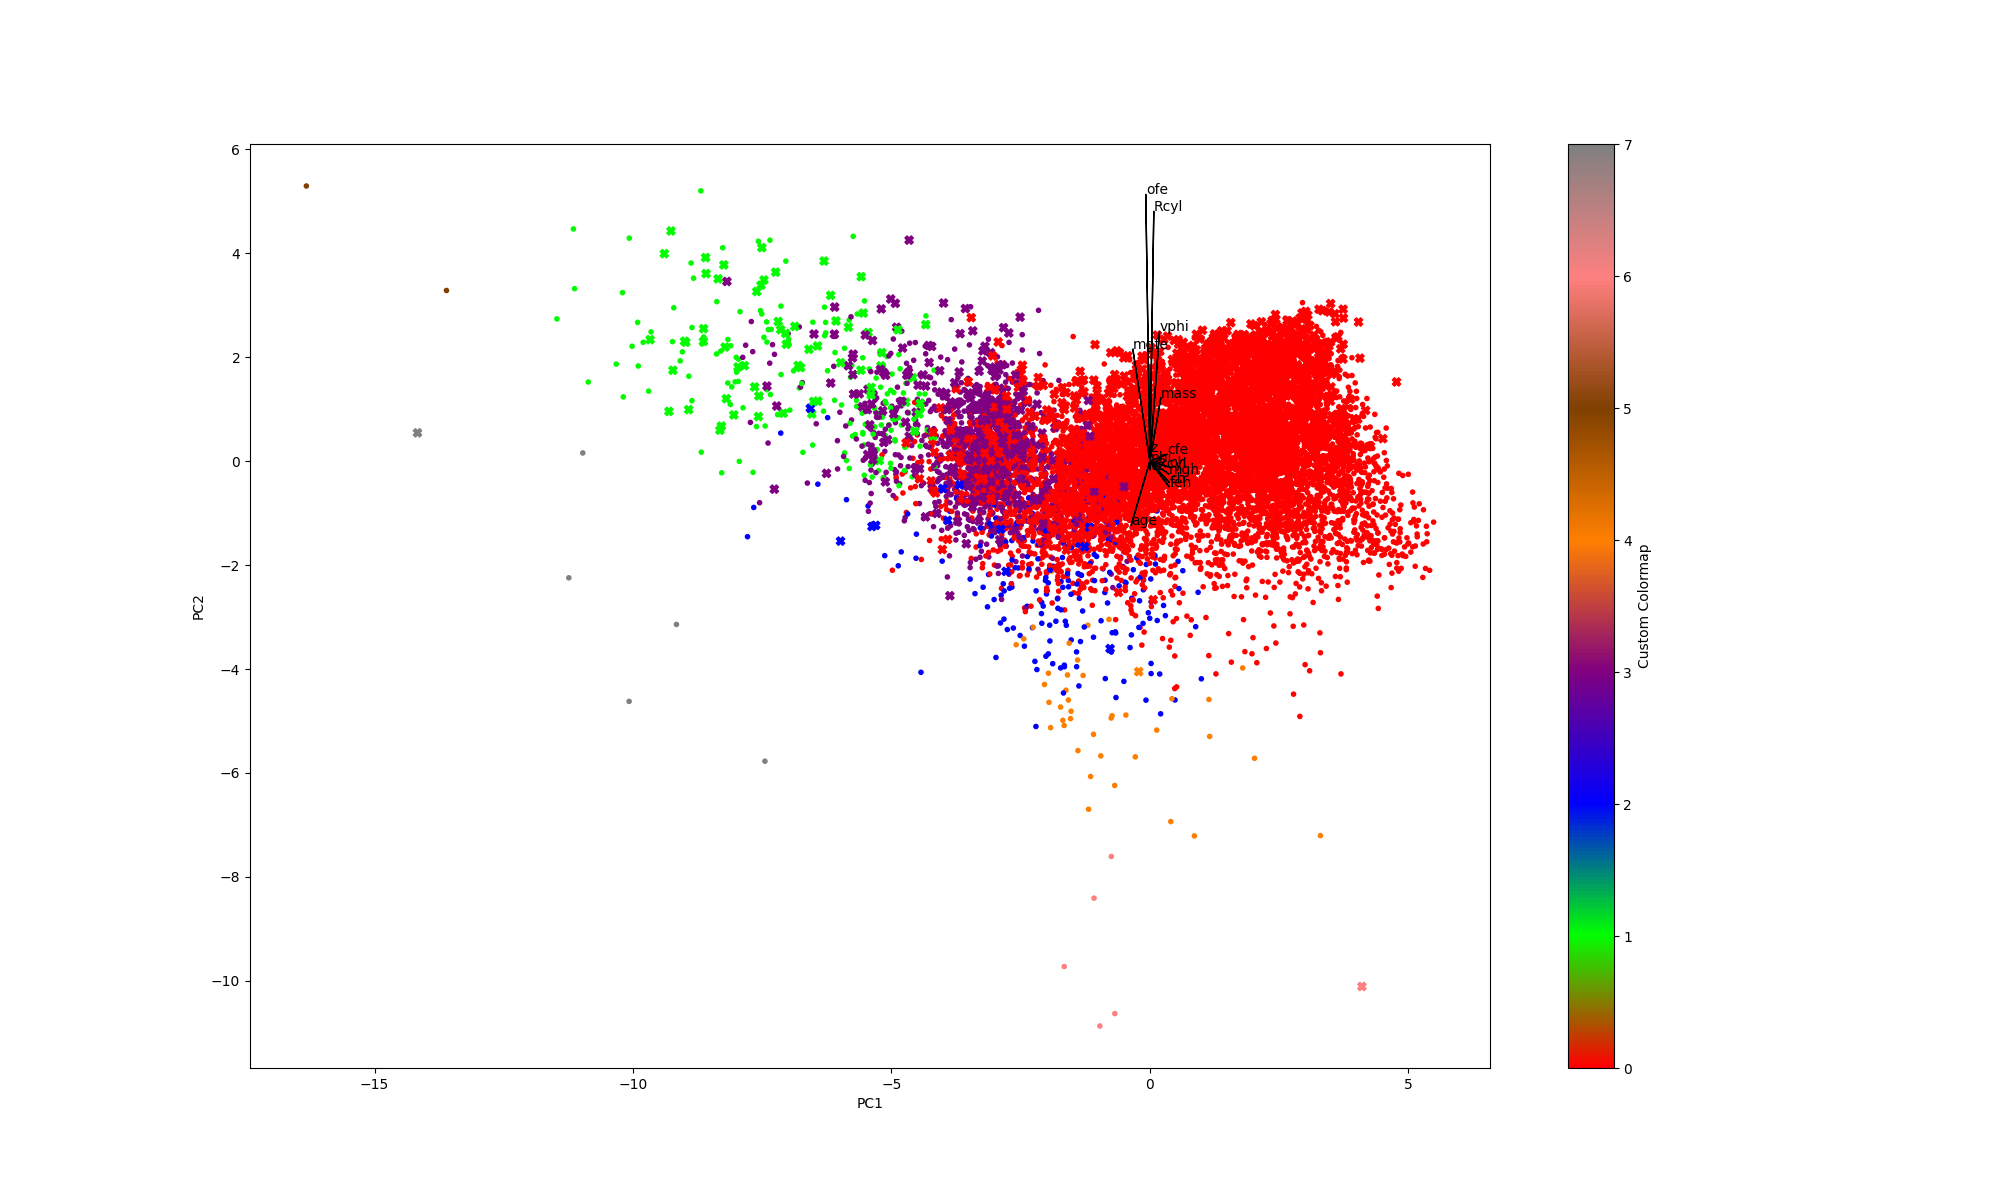
\includegraphics[width=\columnwidth]{Plots/Biplot_with_clustering.png}
    \caption{Scatter Matrix of sample data}
    \label{fig:biplot}
\end{figure}

Using dimensionality reduction does not yield great results either as seen in fig \ref{fig:biplot}, as the clusters don't have well defined lines in a 2d prediction, although this may be due to the high dimensionality data.